\section{Processing fewer blocks}

The complexity of most demanding on-chain operations of the verifier are linear
to proof size. This includes the proof validation and the evaluation of score.
We now present techniques that allow for equivalent operations of constant
complexity.

\textsf{Optimistic schemes.} In smart contracts, in order to
ensure that users comply with the underlying application's rules, certain
actions need to be performed on-chain, e.g.\ verification of data, balance
checks, etc. In a different approach, actions that deviate from the protocol are
reverted after honest users indicate them, not allowing diverging entities to
gain advantages.  Such applications that do not check the validity of actions
by default, but rather depend on the intervention of other users are
characterized ``optimistic''. In the Ethereum community, several projects
~\cite{piza, plasma, rollups-1, rollups-2} have been emerged that incorporate
the notion of \emph{optimistic interactions}. We observe that such a schema can
be embedded into the NIPoPoW protocol, resulting to significant performance gain.

We discussed how the verification in the NIPoPoW protocol is realized in
two phases. In \emph{submit} phase, the verification of the $\pis$ is
performed.  This is necessary in order to prevent adversaries from injecting
blocks that do not belong to the chain, or changing existing blocks. A proof is
valid for submission if it is \emph{structurally correct}. Correctly structured
NIPoPoWs has the following requirements:

\begin{enumerate}
    \item The first block of the proof is the genesis block of the underlying
        blockchain.
    \item Every block has a valid interlink.
\end{enumerate}

Asserting the existence of genesis in the first index of a proof is an
inexpensive operation of constant complexity. However, confirming the interlink
correctness of all blocks is a process of linear complexity to the size of the
proof. Albeit the verification is performed in memory, sufficiently large
proofs result into costly submissions since their validation consist the most
demanding function of \emph{submit} phase. In
Table~\ref{tab:valid-interlink-cost} we display the cost of
\textsf{valid-interlink} function which determines the structural correctness
of a proof in comparison with the overall gas used in \textsf{submit}.

\begin{table}[h]
\begin{tabular}{|c|c|c|}
\hline
\textbf{Process} & \textbf{Gas cost} & \multicolumn{1}{l|}{\textbf{Total \%}} \\ \hline
\textsf{verify-interlink} & 2,200,000         & 53\%                                     \\ \hline
\textsf{submit}           & 4,700,000         & 100\%                                    \\ \hline
\end{tabular}
\caption{Gas usage of \textsf{verify-interlink} compared to the overall
gas consumption of \textsf{submit}.}
\label{tab:valid-interlink-cost}
\vspace*{-5mm}
\end{table}


\newcommand{\dispute}{\emph{dispute\ }} \noindent \textbf{Dispute phase.} We
observe that the addition of a phase in our protocol alleviates the burden of
verifying all elements of the proof by enabling the indication of an individual
incorrect block. This phase, which we term \dispute phase, leverages selective
verification of the submitted proof at a certain index. As a constant
operation, this significantly reduces the gas cost of the verification process.

In the NIPoPoW protocol, when a proof $\pis$ is submitted by $\es$, it is
retrieved by a node $\ec$ from the calldata and the proof is checked for its
validity \emph{off-chain}. The critical observation we make is that in
order to prove a structurally invalid $\pis$, $\ec$ only needs to
indicate the index in which $\pis$ fails the interlink verification. In the
protocol that incorporates \emph{dispute} phase, $\ec$ calls
$\textsf{dispute}$($\pisa$, $i$) for a structurally incorrect proof, where $i$
indicates the disputing index of $\pisa$. Therefore, only one block is
interpreted \emph{on-chain} rather than the entire span of $\pisa$.

Note that, this additional phase does not imply increased rounds of
interactions between $\es$ and $\ec$. If $\pis$ is invalidated in
\emph{dispute} phase, then \emph{contest} phase is skipped. Similarly, if
$\pis$ is structurally correct, but represents a dishonest chain, then $\ec$
proceeds directly to \emph{contest} phase.

In Table~\ref{tab:dispute-cost} we display the gas consumption for
two independent cycles of interactions:
\begin{enumerate}
    \item Phases \emph{submit} and \emph{dispute} for the case in which $\pis$
        is structurally incorrect.
    \item Phases \emph{submit} and \emph{contest} for the case in which
        $\pis$ is structurally correct, but represents a dishonest chain.
\end{enumerate}

\noindent In Algorithm~\ref{alg:dispute-best-level}, we show the implementation
of \emph{dispute} phase. The integration of \emph{dispute} phase leaves
\textsf{contest} unchanged.

\begin{table}
\centering
\begin{tabular}{ccccccc|cc}
            & \textbf{Phase} & \textbf{Gas} &  &              & \textbf{Phase} & \textbf{Gas} & \textbf{Phase} & \textbf{Gas} \\ \cline{2-3} \cline{6-9}
 & submit  & 4.7 &  &  & submit  & 2.2 & submit  & 2.2 \\
 & contest & 4.9 &  &  & dispute & 1.3 & contest & 4.9 \\ \cline{2-3} \cline{6-9}
\textbf{I.} & \textbf{Total} & \textbf{9.6} &  & \textbf{II.} & \textbf{Total} & \textbf{3.5} & \textbf{Total} & \textbf{7.1}
\end{tabular}

\caption{Performance per phase. Gas units are displayed in millions.
\textbf{I}: Gas consumption prior to dispute phase incorporation. \textbf{II}:
Gas consumption for two independent sets of interactions submit/dispute and
submit/contest.}

\label{tab:dispute-cost}
\end{table}


\noindent \textbf{Isolating the best level.} As we discussed, \emph{dispute}
and \emph{contest} phases are mutually exclusive. Unfortunately, the same
constant-time verification as in \emph{dispute} phase cannot be applied in a
contest without increasing the rounds of interactions for the users. However,
we derive a major optimization for \emph{contest} phase by observing the
process of score evaluation.

In NIPoPoWs, after the last common ancestor is found, each fork of the proofs
is evaluated in terms of proof-of-work score. Each level encapsulates different
score of proof-of-work, and the level with the best score is the representative
of the underlying proof. Since the common blocks of the two proofs naturally
gather the same score, only the disjoint portions need to be addressed.
Consequently, the position of the $\lca$ determines the span of the proofs that
will be included in the score evaluation process. Furthermore, it is impossible
to determine the score of a proof in \emph{submit} phase because the position
of $\lca$ is unknown.

After $\pis$ is retrieved from the call data, the score of both proofs is
calculated. This means that, the level in which each proof encapsulates the
most proof-of-work for each proof is known to $\ec$. In the light of this
observation, $\ec$ only submits the blocks which consist the \emph{best level}
of $\pic$. The number of these blocks is constant, as it is determined by the
security parameter $m$, which is irrelevant to the size of the underlying
blockchain. We illustrate the blocks that participate in the formulation of a
proof's score and the best level of contesting proof in
Figure~\ref{fig:score-at-levels}.

The calculation of best level of $\pic$ is an \emph{off-chain} process.
An adversarial $\ec$ is certainly able to dispatch a level of $\pic$ which is
different than the best level. However, this is an irrational action, since
different levels only undermine the score of $\pic$. On the contrary, due to
the consistency property of \emph{hash-and-resumbit}, $\pis$ cannot be altered.
We denote the best level of $\pitr$ as $\pitrl$.

\begin{figure}[H]
    \begin{center}
        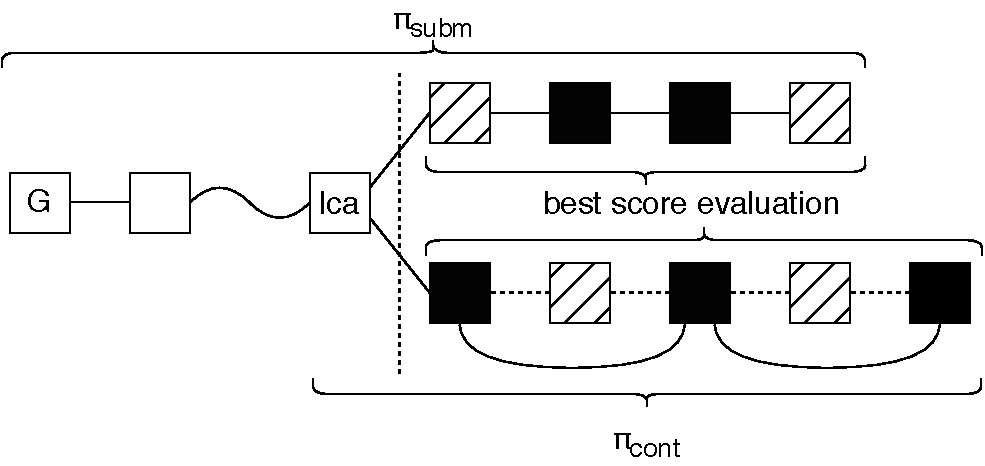
\includegraphics[width=1\columnwidth]{figures/blocks-of-best-level.pdf}
    \end{center}
    \caption{Fork of two proofs. Gray blocks after the lca determine the
    score of each proof. Black blocks belong to the level that
    has the best score. Only black blocks are part of the best level of the
    contesting proof.}
    \label{fig:score-at-levels}
\end{figure}

In Algorithm~\ref{alg:dispute-best-level}, we show the implementation of
\emph{contest} phase under the best-level enhancement.  The utilization of
\emph{best-level} methodology greatly increases the performance of the client,
because the complexity of the majority of $\textsf{contest}$ functions is
related to the size of $\pic$. In Table~\ref{tab:best-level-cost}, we
demonstrate the difference in gas consumption in \emph{contest} phase after
using \emph{best-level}. The performance of most functions is increased by
approximately 85\%. This is due to the fact that the size of $\pic$ is
decreased accordingly. For $m=15$, $\pitrl$ consists of 31 blocks, while
$\pitr$ consists of 200 blocks.  Notably, the calculation of score for $\pitrl$
needs 97\% less gas. We achieve such a discrepancy because the process of score
calculation for multiple levels demands the use of a temporary hashmap which is
a storage structure. In contrast, the evaluation of score of a individual level
is performed entirely in memory.

\begin{table}[]
\begin{tabular}{|c|l|r|r|l|r|r|}
\cline{1-1} \cline{3-4} \cline{6-7}
\textbf{Process} &
   &
  \multicolumn{1}{c|}{\textbf{\begin{tabular}[c]{@{}c@{}}Gas\\ Cost\end{tabular}}} &
  \multicolumn{1}{c|}{\textbf{Total}} &
   &
  \multicolumn{1}{c|}{\textbf{\begin{tabular}[c]{@{}c@{}}Gas\\ Cost\end{tabular}}} &
  \multicolumn{1}{c|}{\textbf{Total}} \\ \cline{1-1} \cline{3-4} \cline{6-7}
  \textsf{valid-interlinks} &            & 900,000   & 18\%  &             & 120,000   & 10\%  \\ \cline{1-1} \cline{3-4} \cline{6-7}
  \textsf{minimal-fork}     &            & 1,900,000 & 39\%  &             & 275,000   & 18\%  \\ \cline{1-1} \cline{3-4} \cline{6-7}
  \textsf{score} (p1)       &            & 750,000   & 16\%  &             & 750,000   & 51\%  \\ \cline{1-1} \cline{3-4} \cline{6-7}
  \textsf{score} (p2)       &            & 950,000   & 19\%  &             & 20,000    & 1\%   \\ \cline{1-1} \cline{3-4} \cline{6-7}
other            &            & 400,000   & 8\%   &             & 300,000   & 20\%  \\ \cline{1-1} \cline{3-4} \cline{6-7}
\textsf{contest}          & \textbf{I} & 4,900,000 & 100\% & \textbf{II} & 1,465,000 & 100\% \\ \cline{1-1} \cline{3-4} \cline{6-7}
\end{tabular}
\caption{Gas usage in contest. I: before utilizing best level. II: after
utilizing best level.}
\label{tab:best-level-cost}
\end{table}


In Figure ~\ref{fig:dispute-best-level}, we illustrate the performance gain of
the client using \emph{dispute} phase and the best-level contesting proof. The
aggregated gas consumption of \emph{submit} and \emph{contest} phases is
reduced to 3,500,000 gas. This is critical threshold regarding applicability of
the contract, since a cycle of interactions now effortlessly fits inside a
single the Ethereum block.

\begin{algorithm}
    \caption{\label{alg:dispute-best-level}The \textsf{NIPoPoW} client enhanced
        with dispute phase and best-level contesting}

    \begin{algorithmic}[1]

    \Contract{crosschain}
    \State $\textsf{events} \gets \bot;$ $\genesis \gets \bot$
    \Function{\sf initialize}{$\genesis_{remote}$}
        \State $\genesis$ $\gets \genesis_{remote}$
    \EndFunction
    \Function{\sf submit}{$\pis$, $e$}
        \State \textsf{require}($\pis$[0] = $\genesis$)
        \State \textsf{require}($\textsf{events$[e]$} = \bot$)
        \State \textsf{events$[e]$.hash} $\gets$ \textsf{H}($\pis$)
        \State \textsf{events$[e]$.pred} $\gets$
        \textsf{evaluate-predicate}(\textsf{$\pis$}, $e$)
    \EndFunction
    \Function{\sf dispute}{$\pisa$, $e$, $i$}
        \Comment{$i$: dispute index}
        \State \textsf{require}(\textsf{events}$[e]$ $\ne$ $\bot$)
        \State \textsf{require}(\textsf{events$[e]$.hash} $=$ \textsf{H}($\pisa$))
        \State \textsf{require}($\neg \textsf{valid-single-interlink}(\pis, i)$)
        \State \textsf{events$[e]$} $\gets$ $\bot$
    \EndFunction
    \Function{\sf valid-single-interlink}{$\pi$, $i$}
        \State $l\gets\pi[i].\mathsf{level}$
        \If{$\pi[i{+}1].\mathsf{intelink}[l] = \pi[i]$}
        \State \Return true
        \EndIf
        \State \Return false
    \EndFunction
    \Function{\sf contest}{$\pisa$, $\pitrl$, $e$, $f$}
        \State \textsf{require}($\pitrl$[0] = $\pisa[f]$)
        \State \textsf{require}(\textsf{events}$[e]$ $\ne$ $\bot$)
        \State \textsf{require}(\textsf{events$[e]$.hash} $=$ \textsf{H}($\pisa$))
        \State \textsf{require}(\textsf{valid-interlinks}($\pitrl$))
        \State \textsf{require}(\textsf{minimal-fork}($\pisa$,
        $\pitrl$, $f$))
        \State \textsf{require}(\textsf{score-at-level}($\pitrl$)
        $>$ \textsf{score}($\pisa[f{:}]$))
        \State \textsf{events$[e]$.pred} $\gets$
            \textsf{evaluate-predicate}($\pitrl$, $e$)
    \EndFunction
    \Function{\sf score-at-level}{$\pi$}
        \State $l \gets \pi[-1].\textsf{level}$
        \Comment{pick proof level from a block}
        \State $score \gets 0$
        \Comment{set score counter to 0}
        \For{b in $\pi$}
            \State \textsf{require}(b.\textsf{level} = $l$)
            \State $score \gets score {+} 2^l$
        \EndFor
        \State \Return{score}
    \EndFunction
    \EndContract
    \vskip8pt
    \end{algorithmic}
\end{algorithm}



\begin{figure}[!h]
    \begin{center}
        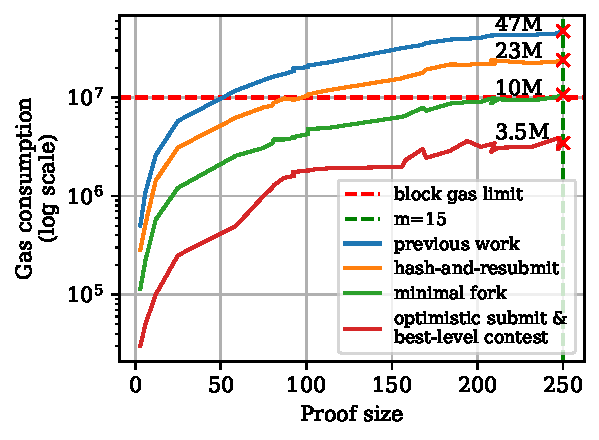
\includegraphics[width=1\columnwidth]{figures/dispute-best-level.pdf}
    \end{center}
    \caption{Performance improvement using optimistic schema in submit phase
        and best level proof in contesting proof (lower is better). The gas
        consumption is decreased by approximately 65\%.}
    \label{fig:dispute-best-level}
\end{figure}
